\section{Parallelization performance}
\label{sec:dsmc_parallelization_performance}
After the code is parallelized, the total computation time needed to perform a simulation is obviously not reduced. There are still as many collisions as before as the physical problem is identical. The idea is to do many of the calculations at the same time so that the total \textit{real} time we actually wait is reduced. Parallelizing is of course not \textit{free} as we need more logic to let the processors communicate with each other (exchanging particles and waiting for each other to finish each time step). As the number of processors increases, the total computation time \textit{per processor} is reduced, but the time spent on communication often increases. We will measure what's called \textit{parallel scalability} which indicates how efficient a program is when the number of processors is increased. There are two different kinds of scalability; weak and strong scaling
\begin{itemize}
	\item strong scaling is how the computation time changes with an increased number of processors on a fixed system size, whereas the
	\item weak scaling is how the computation time changes with an increased number of processors on a fixed system size \textit{per processor}.
\end{itemize}


\section{Results for simple geometries}
\label{sec:results_for_simple_geometries}
In this section, we will study flow in simple geometries where the theoretical permeability is well known. The expression for the permeability is only valid for small Knudsen numbers (which we called the absolute permeability; the permeability for fluids in the continuum limit), so it is a perfect test case for the Knudsen correction factor $f_c$ in equation \eqref{eq:knudsen_correction}. 

\subsection{Flow in a cylinder, varying Knudsen number}
We have induced flow in a cylinder with radius \unit{0.45}{\micro\meter} with an applied acceleration corresponding to a pressure difference $\Delta P = 1.1P_0$, where $P_0$ is the ideal gas pressure at \unit{300}{\kelvin}. We want to vary the Knudsen number which was defined as
\begin{align}
	\text{Kn} = \frac{\lambda}{L} = \frac{1}{\sqrt 2 \pi d^2 \rho_n L}
\end{align}
where $L$ is the length of the cylinder, $\lambda$ is the mean free path. We have used equation \eqref{eq:mean_free_path} in the last expression so that we can choose the Knudsen number through the density
\begin{align}
	\rho_n(\text{Kn}) = \frac{1}{\sqrt 2 \pi d^2 \text{Kn}L}.
\end{align}
We expect an apparent permeability satisfying the Knudsen correction
\begin{align}
	k_a = k_\infty f_c = k_\infty[1 + \alpha(\text{Kn})\text{Kn}]\left[1 + {4\text{Kn}\over 1 + \text{Kn}}\right].
\end{align}
The analytical absolute permeability for a cylinder with radius $r$ is given by\cite{karniadakis2005microflows}
\begin{align}
	\label{eq:permeability_cylinder}
	k_\infty = {r^2\over 8},
\end{align}
which gives the following prediction for the apparent permeability
\begin{align}
	k_a = [1 + \alpha(\text{Kn})\text{Kn}]\left[1 + {4\text{Kn}\over 1 + \text{Kn}}\right] {r^2\over 8}.
\end{align}
In figure \ref{fig:one_cylinder_varying_knudsen} we have plotted the measured permeability as a function of Knudsen number. We see that the 

\begin{figure}[h]
\begin{center}
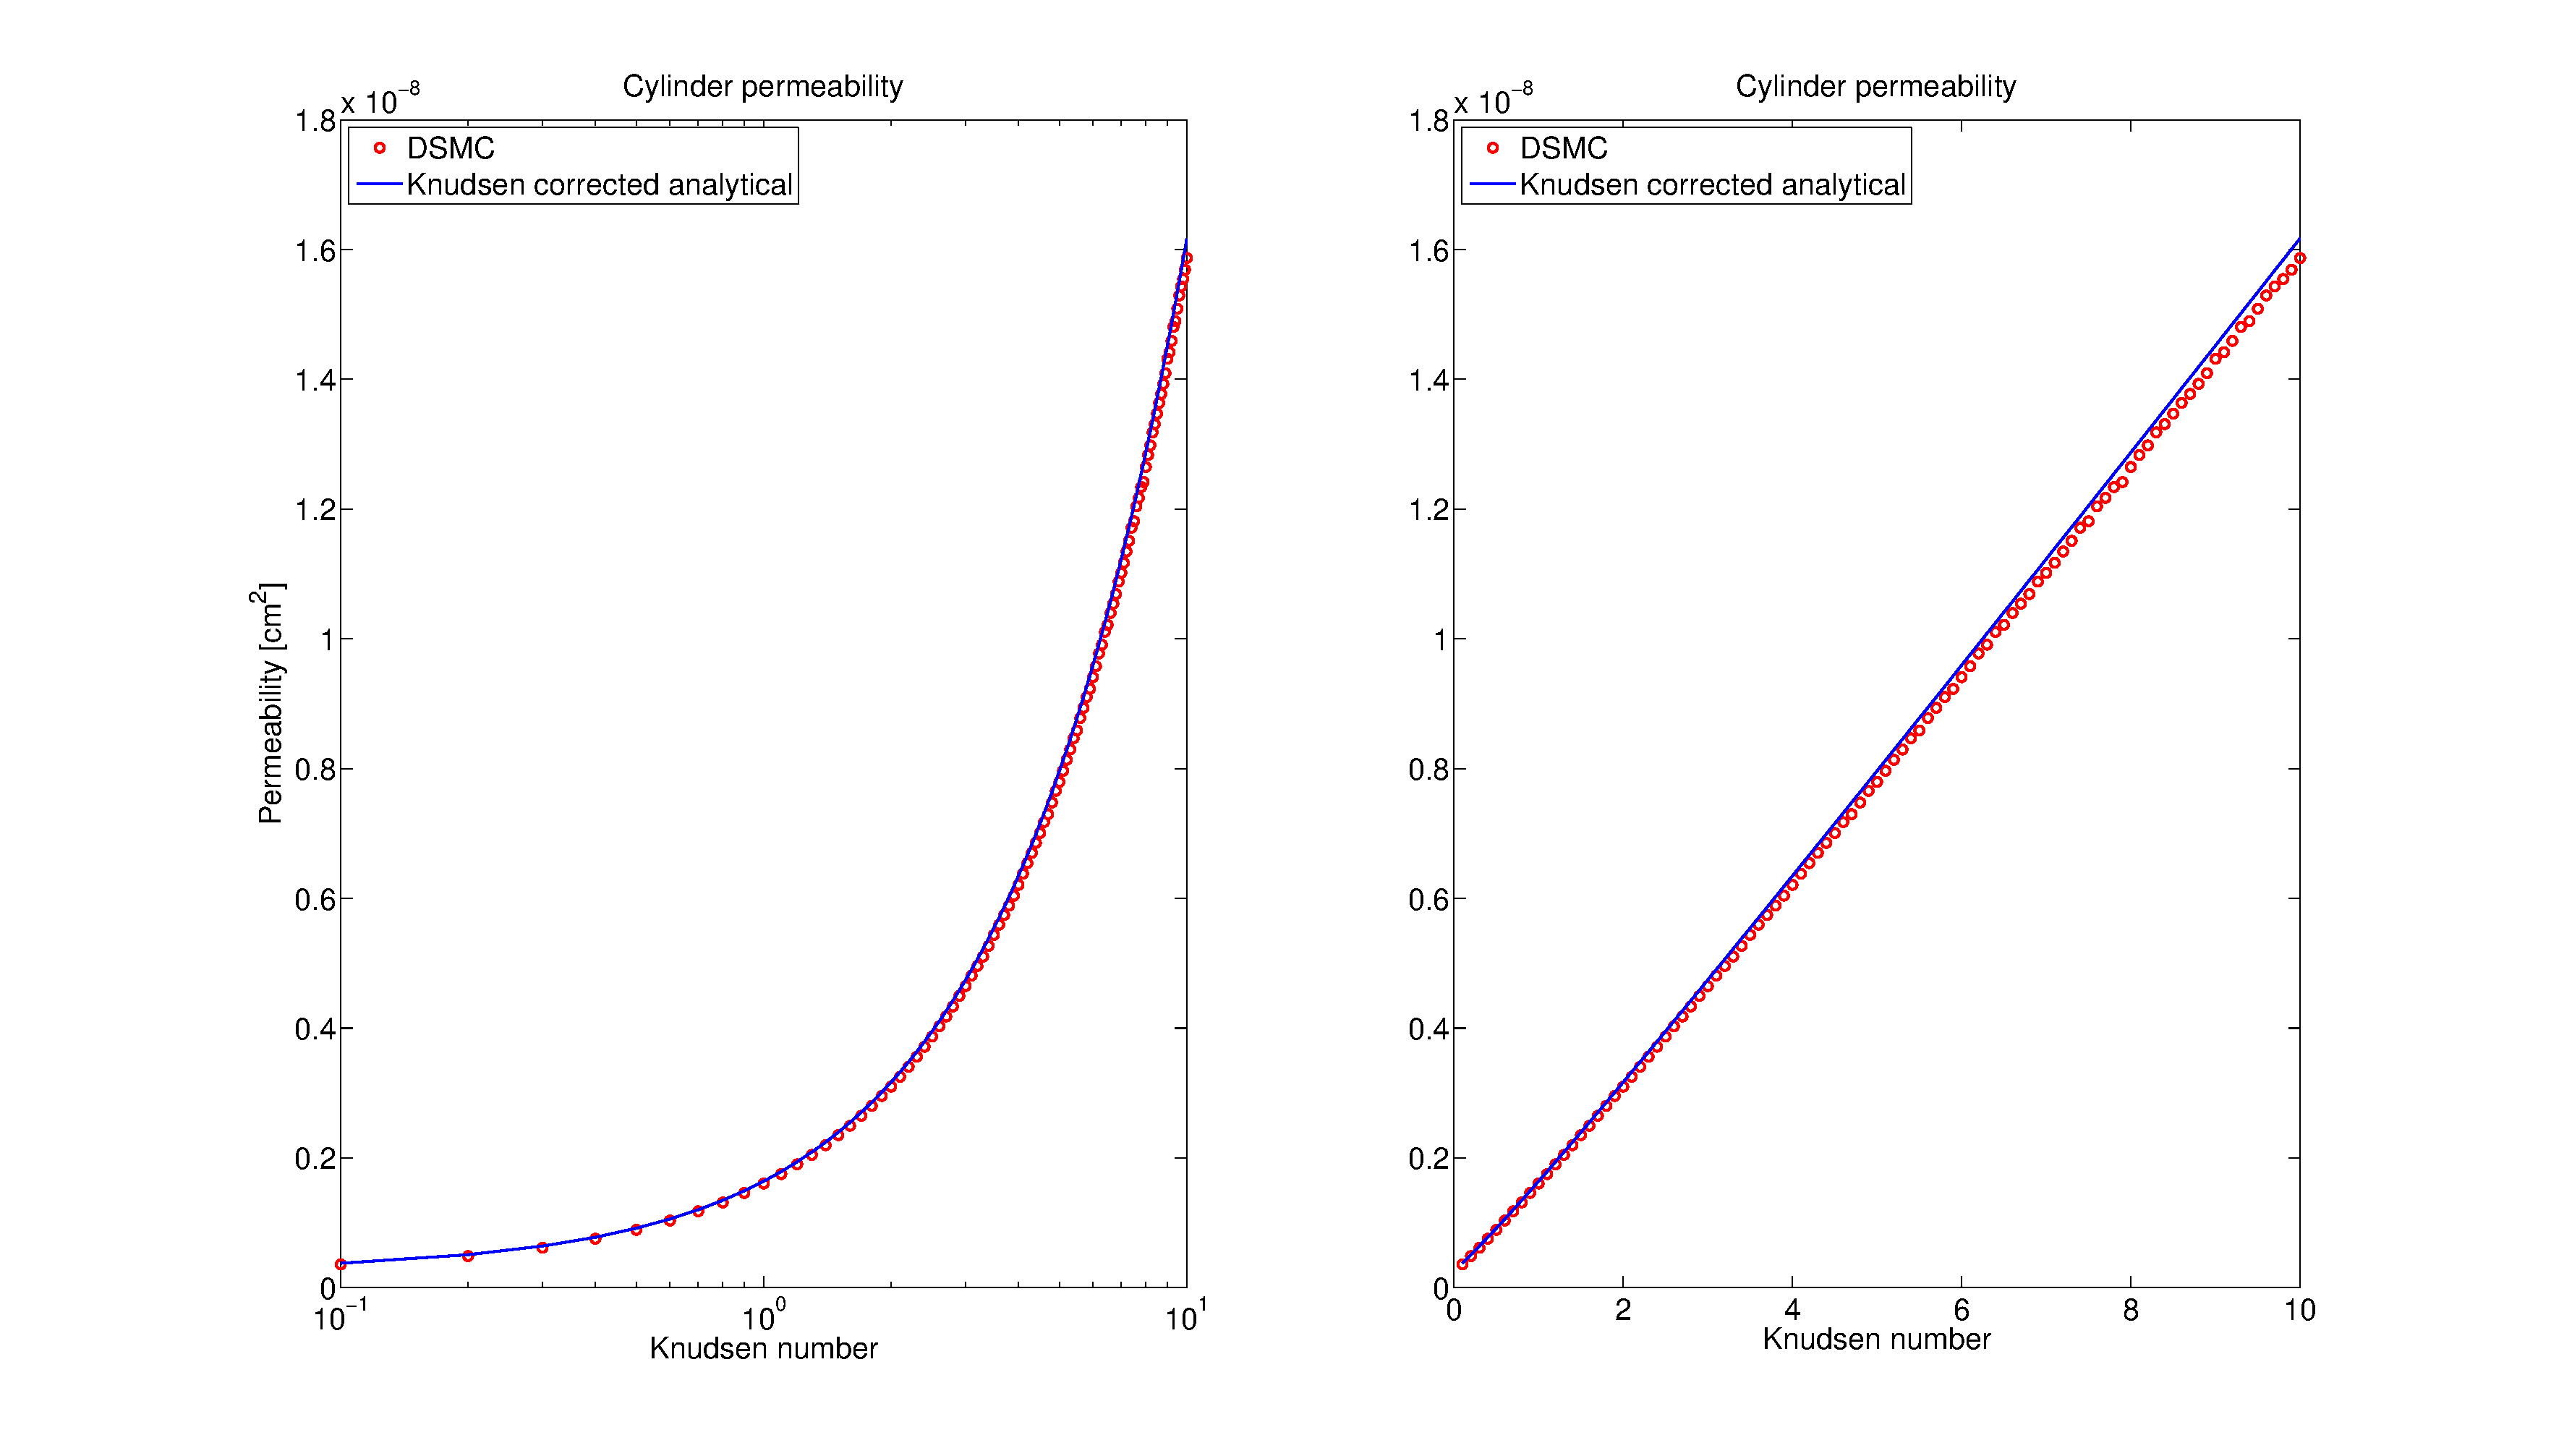
\includegraphics[width=\textwidth, trim=0cm 0cm 0cm 0cm, clip]{DSMC/figures/cylinder_knudsen_permeability.eps}
\end{center}
\caption{Permeability as a function of Knudsen number for a cylinder with radius \unit{0.45}{\micro\meter} and length \unit{1}{\micro\meter} with an applied pressure difference $\Delta P = 1.1P_0$ ($P_0$ being the ideal gas pressure). We control the Knudsen number by varying the density. The blue line is the Knudsen corrected analytical solution from \cite{karniadakis2005microflows}. The DSMC results confirm that the Knudsen correction factor works very well for a system with a well defined Knudsen number.}
\label{fig:one_cylinder_varying_knudsen}
\end{figure}

\subsection{Flow in a cylinder, varying radius}
If we instead keep the Knudsen number constant ($\text{Kn}=1.0$), we can vary the radius to verify equation \eqref{eq:permeability_cylinder}. We have studied radii in the range \unit{0.1}{\micro\meter} to \unit{0.45}{\micro\meter} with the same pressure difference as in the previous simulation ($\Delta P = 1.1P_0)$. In figure \ref{fig:one_cylinder_varying_radii_result} we have plotted the measured permeability as a function of cylinder radius. The straight line confirms the quadratic dependency in equation \eqref{eq:permeability_cylinder}.
\begin{figure}[h]
\begin{center}
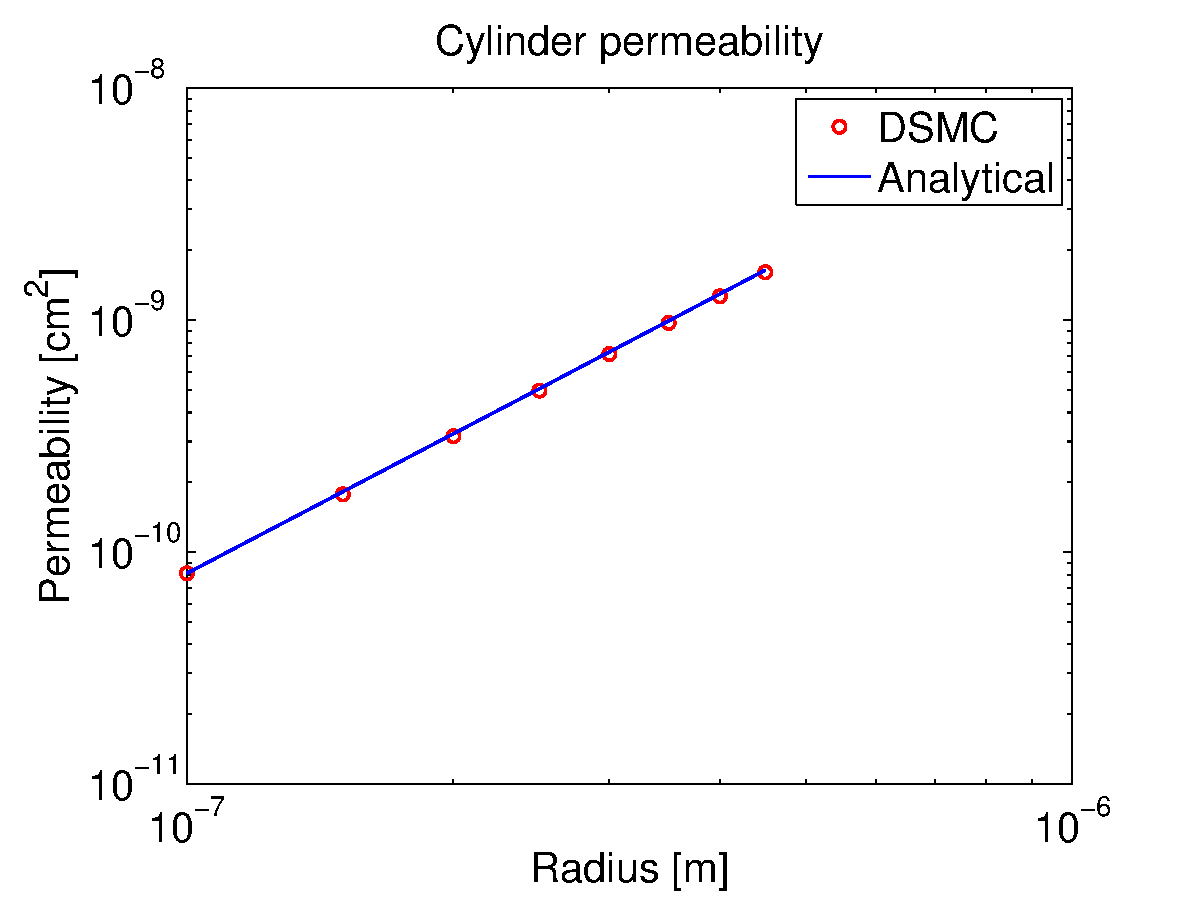
\includegraphics[width=\textwidth, trim=0cm 0cm 0cm 0cm, clip]{DSMC/figures/cylinder_radius_permeability.eps}
\end{center}
\caption{Logarithmic plot of the permeability for different cylinders with radii in the range $0.1 \mu m$ to $0.45 \mu m$ with an applied pressure difference $\Delta P = 1.1P_0$. The blue line is the Knudsen corrected analytical solution from \cite{karniadakis2005microflows}.}
\label{fig:one_cylinder_varying_radii_result}
\end{figure}
\section{Results for complicated geometries}
\subsection{Randomly packed spheres}
Through the Carman-Kozeny equation, we can theoretically predict the permeability for randomly packed spheres 
\begin{align}
	k = {a^2 \over 9K} {\phi^3 \over (1 - \phi)^2},
\end{align}
where $\phi$ is the porosity, $a$ is the sphere radius and $K$ Kozeny constant which is experimentally measured to be around five\cite{carman1937fluid}. This theoretical result has been verified to predict permeabilities in experiments, but at micrometer scale, we expect deviations. 
